A montagem do tambor, com os esforços atuantes está ilustrada abaixo:

\begin{figure}[H]
  \centering
  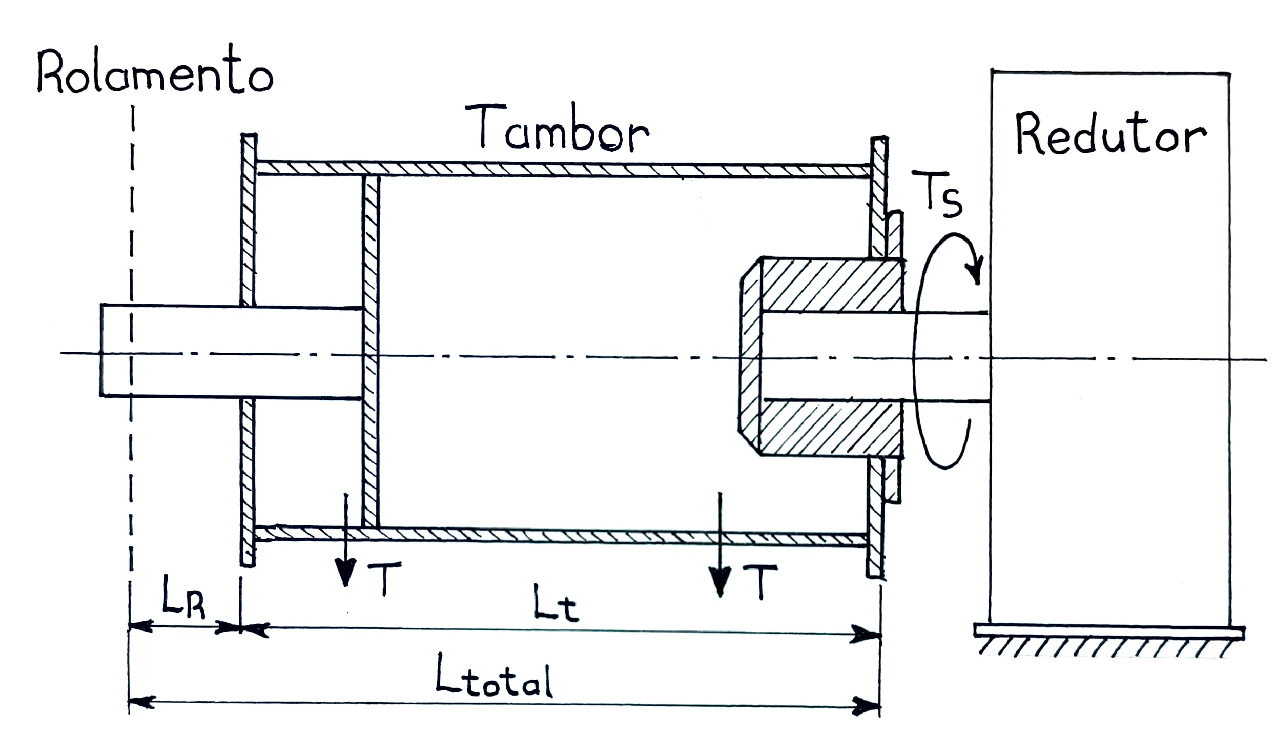
\includegraphics[width=0.8\textwidth]{content/sections/03_sistema_de_elevacao/sections/04_projeto_do_tambor/sections/01_modelagem_estatica_do_tambor/figures/tambor_redutor.pdf}
  \caption{Representação da montagem do tambor com o redutor (Autor)}
  \label{fig:montagem_tambor}
\end{figure}

A estrutura do tambor pode ser modelada como uma viga bi apoiada, com o peso do tambor e do cabo de aço atuando em forma de carga distribuída, conforme ilustrado abaixo:

\begin{figure}[H]
  \centering
  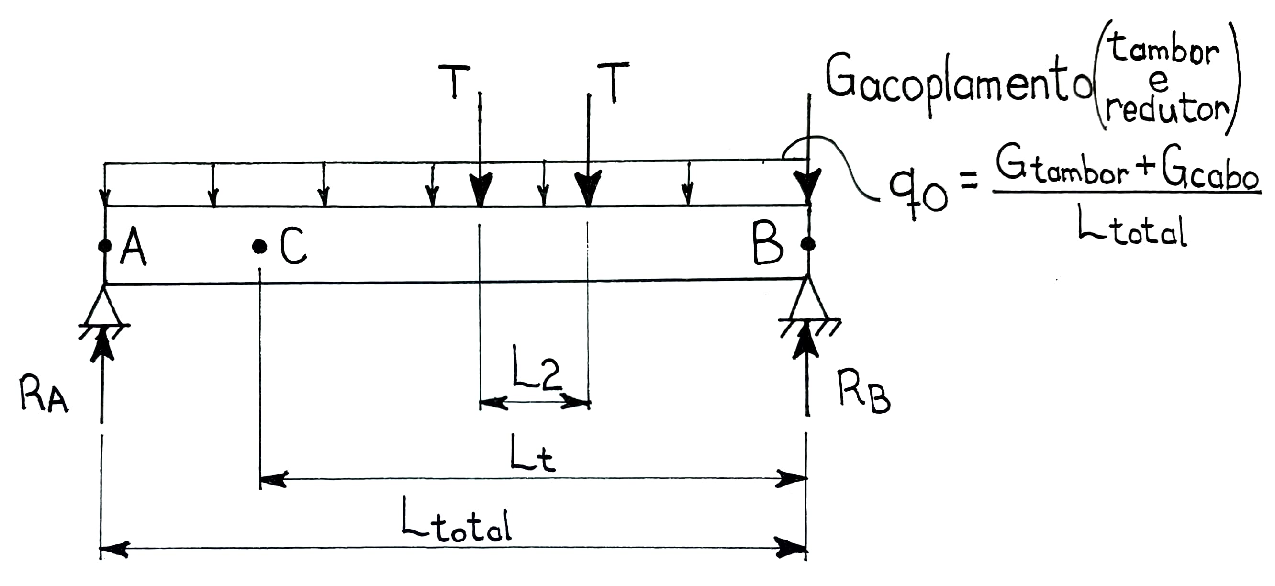
\includegraphics[width=0.8\textwidth]{content/sections/03_sistema_de_elevacao/sections/04_projeto_do_tambor/sections/01_modelagem_estatica_do_tambor/figures/modelagem_tambor.pdf}
  \caption{Modelagem estática do tambor (Autor)}
  \label{fig:modelagem_tambor}
\end{figure}

\subsubsection{Cargas}

A tração no cabo de aço, conforme calculada na Seção \ref{sec:forca_de_tracao_no_cabo}, é de \SI{25377.8}{\newton}.

O peso do acoplamento redutor-tambor, obtido no catálogo (Tabela \ref{tab:dados_acoplamento_tambor}), é de \SI{54}{\kilogram}, equivalente a \SI{540}{\newton}.

O peso do tambor, conforme calculado na Seção \ref{sec:peso_do_tambor}, é de \SI{6611.851}{\newton}.

Já o peso do cabo de aço, conforme calculado na Seção \ref{sec:peso_do_cabo_de_aco}, é de \SI{978.48}{\newton}.

A carga distribuída considerada na modelagem estática é dada por:

\begin{equation}
  q_o = \frac{G_{\text{tambor}} + G_{\text{cabo}}}{L_{\text{total}}}
  \label{eq:carga_distribuida_tambor}
\end{equation}

\begin{align*}
  q_o & = \frac{\num{6611.85} + \num{978.48}}{\num{2.212}} \\
  q_o & = \boxed{\SI{3431.4}{\newton\per\meter}}
\end{align*}

As cargas atuantes consideradas no dimensionamento do tambor estão resumidas abaixo:

\begin{table}[H]
  \centering
  \caption{Cargas atuantes no tambor}
  \label{tab:cargas_atuantes_tambor}
  \begin{tabularx}{\textwidth}{>{\centering\arraybackslash}X>{\centering\arraybackslash}X>{\centering\arraybackslash}X}
    \toprule
    Descrição                          & Símbolo                  & Valor                          \\
    \midrule
    Tração no cabo de aço              & $T$                      & \SI{25377.8}{\newton}          \\
    Peso do acoplamento redutor-tambor & $G_{\text{acoplamento}}$ & \SI{540}{\newton}              \\
    Peso do tambor                     & $G_{\text{tambor}}$      & \SI{6611.85}{\newton}          \\
    Peso do cabo de aço                & $G_{\text{cabo}}$        & \SI{978.48}{\newton}           \\
    Carga distribuída                  & $q_o$                    & \SI{3431.4}{\newton\per\meter} \\
    \bottomrule
  \end{tabularx}
\end{table}

\subsubsection{Distâncias}

As distâncias consideradas na modelagem estática são:

\begin{table}[H]
  \centering
  \caption{Distâncias consideradas na modelagem estática}
  \label{tab:distancias_consideradas_modelagem_estatica}
  \begin{tabularx}{\textwidth}{>{\centering\arraybackslash}X>{\centering\arraybackslash}X>{\centering\arraybackslash}X}
    \toprule
    Descrição                             & Símbolo            & Valor              \\
    \midrule
    Espaçamento central entre as ranhuras & $L_2$              & \SI{0.2}{\meter}   \\
    Comprimento do tambor                 & $L_t$              & \SI{2.112}{\meter} \\
    Comprimento total                     & $L_{\text{total}}$ & \SI{2.212}{\meter} \\
    \bottomrule
  \end{tabularx}
\end{table}

\subsubsection{Diagrama de corpo livre}

Com base nas cargas e distâncias consideradas, o diagrama de corpo livre (DCL) do tambor é ilustrado abaixo:

\begin{figure}[H]
  \centering
  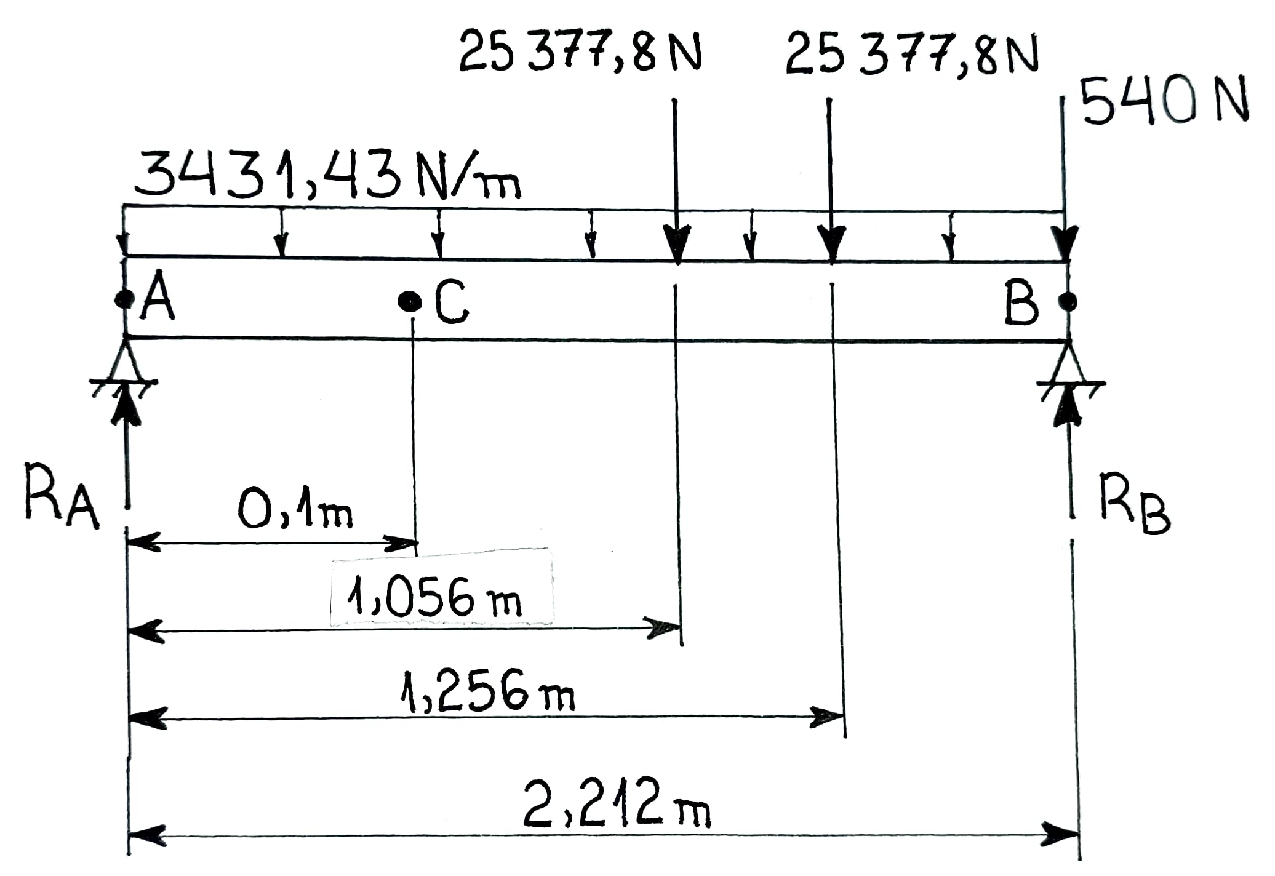
\includegraphics[width=0.8\textwidth]{content/sections/03_sistema_de_elevacao/sections/04_projeto_do_tambor/sections/01_modelagem_estatica_do_tambor/figures/dcl_tambor.pdf}
  \caption{DCL do tambor (Autor)}
  \label{fig:dcl_tambor}
\end{figure}

\subsubsection{Reações de apoio}

Utilizando as equações de equilíbrio, as reações de apoio podem ser calculadas.

Os momentos atuantes no ponto A são:

\begin{equation*}
  \num{2.212} \cdot R_B
\end{equation*}

\begin{equation*}
  - \num{3431.43} \cdot \frac{\num{2.212}}{2} \cdot \num{2.212} = \SI{-8394.9}{\newton\meter}
\end{equation*}

\begin{equation*}
  - \num{1.056} \cdot \num{25377.8} = \SI{-26798.96}{\newton\meter}
\end{equation*}

\begin{equation*}
  - \num{1.256} \cdot \num{25377.8} = \SI{-31874.52}{\newton\meter}
\end{equation*}

\begin{equation*}
  - \num{2.212} \cdot 540 = \SI{-1194.48}{\newton\meter}
\end{equation*}

\vspace{1em}

Aplicando nas equações de equilíbrio, tem-se:

\begin{flalign*}
   & \sum M_A = 0                                                                         &  & \\
   & \num{2.212} R_B - \num{8394.9} - \num{26798.96} - \num{31874.52} - \num{1194.48} = 0 &  &
\end{flalign*}

\begin{equation}
  \num{2.212} R_B - \num{68262.86} = 0
  \label{eq:sum_ma_tambor}
\end{equation}

\vspace{1em}

\begin{flalign*}
   & \sum F_y = 0                                                                  &  & \\
   & R_A + R_B - \num{3431.43} \cdot \num{2.212} - 2 \cdot \num{25377.8} - 540 = 0 &  &
\end{flalign*}

\begin{equation}
  R_A + R_B - \num{58885.92} = 0
  \label{eq:sum_fy_tambor}
\end{equation}

\vspace{1em}

Desenvolvendo a equação \eqref{eq:sum_ma_tambor}, tem-se:

\begin{align*}
  R_B & = \frac{\num{68262.86}}{\num{2.212}} \\
  R_B & = \boxed{\SI{30860.24}{\newton}}
\end{align*}

\vspace{1em}

Substituindo o valor de $R_B$ na equação \eqref{eq:sum_fy_tambor}, tem-se:

\begin{align*}
  R_A & = \num{58885.92} - \num{30860.24} \\
  R_A & = \boxed{\SI{28025.68}{\newton}}
\end{align*}

\vspace{1em}

\subsubsection{Funções de singularidade}

Para obter as equações dos esforços internos de força cortante e momento fletor, utilizou-se o método das funções de singularidade de Macaulay.

\begin{align*}
  V(x) & = -\num{3431.43} \left<x\right>^1 + \num{28025.68} \left<x\right>^0 - \num{25377.8} \left<x - \num{1.056}\right>^0 \rightarrow                                        \\
       & \quad - \num{25377.8} \left<x - \num{1.256}\right>^0 - 540 \left<x - \num{2.212}\right>^0 - \num{30860.24} \left<x - \num{2.212}\right>^0 \left[ \si{\newton} \right]
\end{align*}

\begin{align*}
  M(x) & = -\frac{\num{3431.43}}{2} \left<x\right>^2 + \num{28025.68} \left<x\right>^1 - \num{25377.8} \left<x - \num{1.056}\right>^1 \rightarrow                                    \\
       & \quad - \num{25377.8} \left<x - \num{1.256}\right>^1 - 540 \left<x - \num{2.212}\right>^1 - \num{30860.24} \left<x - \num{2.212}\right>^1 \left[ \si{\newton\meter} \right]
\end{align*}

Desenvolvendo as funções de singularidade, é possível extrair as equações para cada segmento da viga:

\[
  V(x) =
  \begin{cases}
    -\num{3431.43} x + \num{28025.68} & 0 \le x \le \SI{1.056}{\meter}                  \\
    -\num{3431.43} x + \num{2647.88}  & \SI{1.056}{\meter} \le x \le \SI{1.256}{\meter} \\
    -\num{3431.43} x - \num{22729.92} & \SI{1.256}{\meter} \le x \le \SI{2.212}{\meter}
  \end{cases}
  \quad \left[ \si{\newton} \right]
\]

\[
  M(x) =
  \begin{cases}
    -\num{1715.72} x^2 + \num{28025.68} x                  & 0 \le x \le \SI{1.056}{\meter}                  \\
    -\num{1715.72} x^2 + \num{2647.88} x + \num{26798.96}  & \SI{1.056}{\meter} \le x \le \SI{1.256}{\meter} \\
    -\num{1715.72} x^2 - \num{22729.92} x + \num{58673.47} & \SI{1.256}{\meter} \le x \le \SI{2.212}{\meter}
  \end{cases}
  \quad \left[ \si{\newton\meter} \right]
\]

\subsubsection{Diagramas de esforço cortante e momento fletor}

Aplicando as equações ao longo do comprimento da viga, tem-se o seguinte diagrama de esforços internos:

\begin{figure}[H]
  \centering
  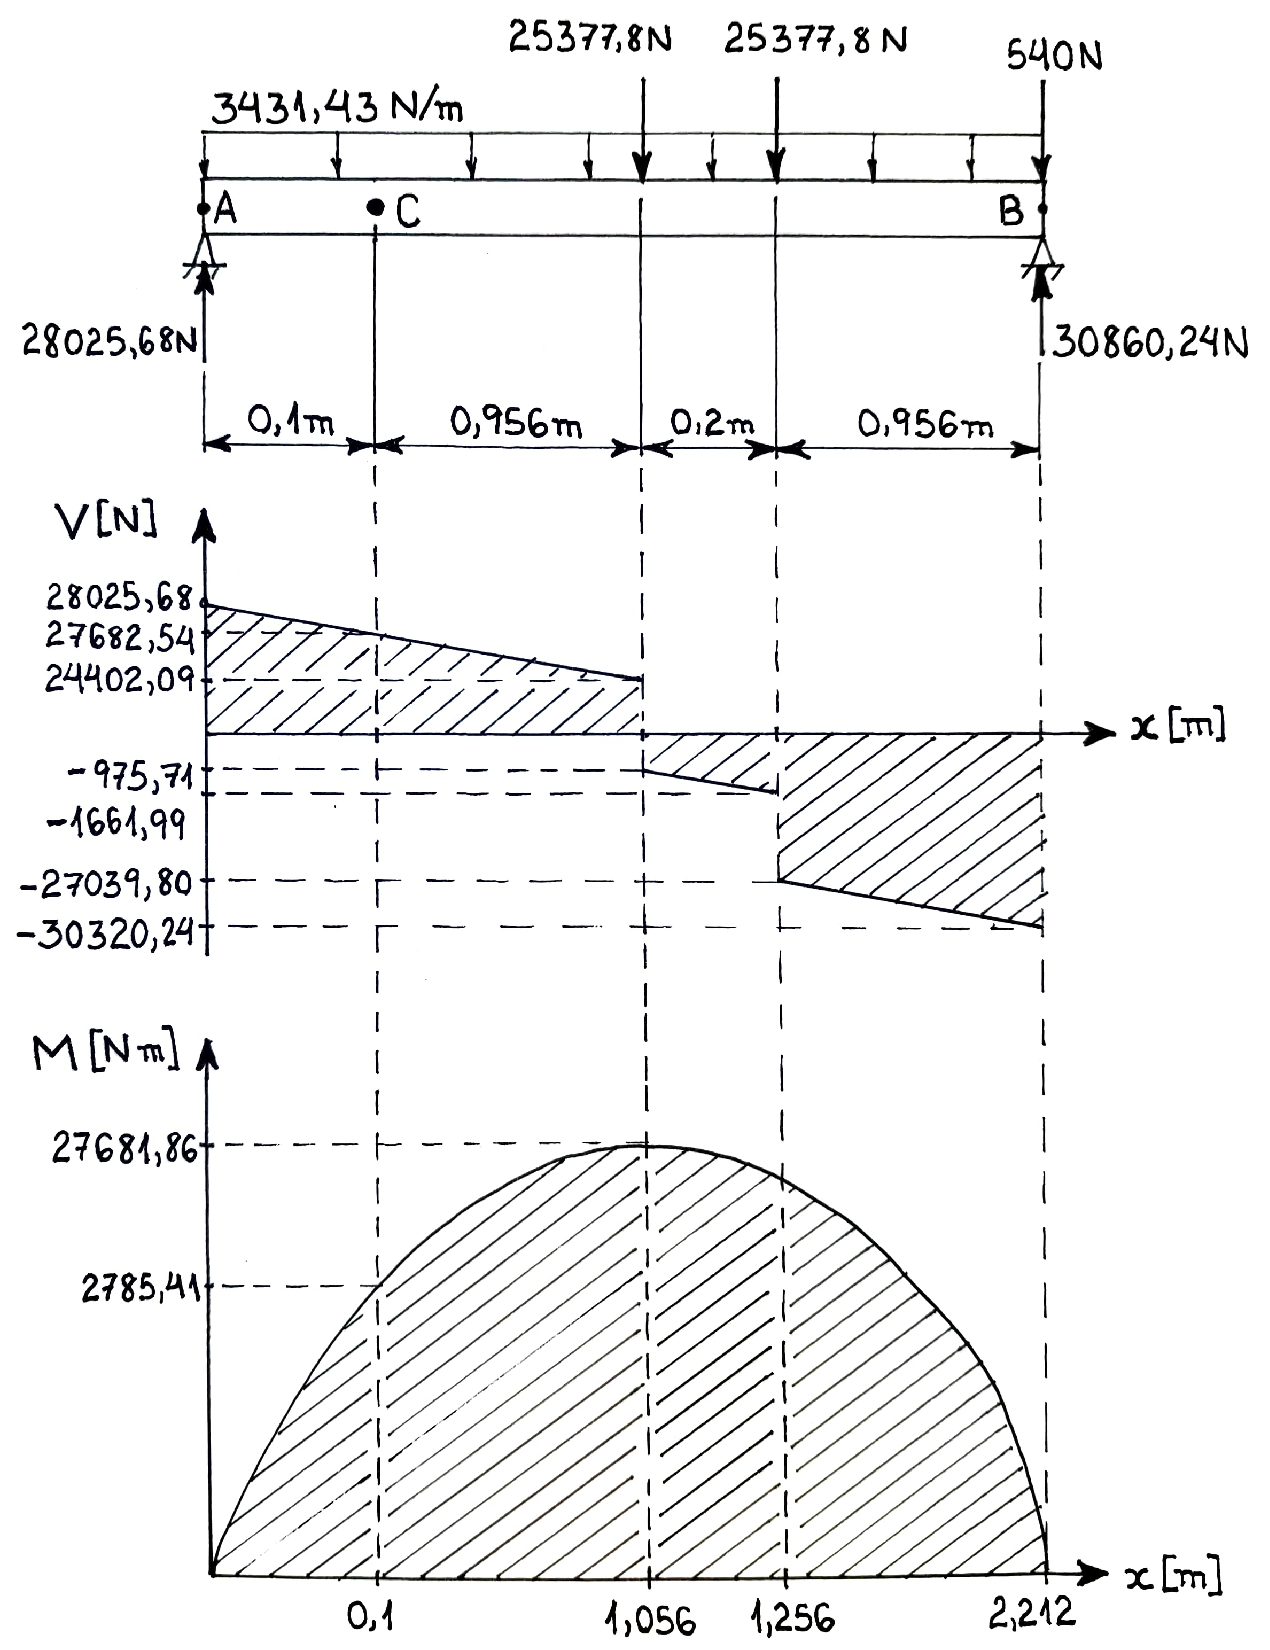
\includegraphics[width=0.8\textwidth]{content/sections/03_sistema_de_elevacao/sections/04_projeto_do_tambor/sections/01_modelagem_estatica_do_tambor/figures/diagrama_tambor.pdf}
  \caption{Diagrama de esforços internos do tambor (Autor)}
  \label{fig:diagrama_tambor}
\end{figure}

Analisando o diagrama, tem-se que o momento fletor máximo no tambor ocorre na posição $x = \SI{1.056}{\meter}$ e a força cortante máxima no tambor ocorre na posição $x = \SI{2.212}{\meter}$.

Assim, é possível extrair os valores de momento fletor máximo e de força cortante máxima no tambor, bem como o momento fletor e a força cortante no eixo (posição $x = \SI{0.1}{\meter}$). Os dados obtidos são:

\begin{table}[H]
  \centering
  \caption{Dados de esforços internos do tambor}
  \label{tab:dados_esforcos_tambor}
  \begin{tabularx}{\textwidth}{>{\centering\arraybackslash}X>{\centering\arraybackslash}X>{\centering\arraybackslash}X}
    \toprule
    Descrição                        & Símbolo   & Valor                        \\
    \midrule
    Momento fletor máximo no tambor  & $M_{f_t}$ & \SI{27681.86}{\newton\meter} \\
    Força cortante máxima no tambor  & $V_t$     & \SI{30320.24}{\newton}       \\
    Momento fletor no eixo do tambor & $M_{f_e}$ & \SI{2785.41}{\newton\meter}  \\
    Força cortante no eixo do tambor & $V_e$     & \SI{27682.54}{\newton}       \\
    \bottomrule
  \end{tabularx}
\end{table}
